\documentclass[0_main]{subfiles}

\begin{document}

\ifEn
    \subsection{Representative Quasi-Newton Update Rules}
\else
    \subsection{代表的な準ニュートン更新公式}
\fi

\ifEn
    Given $B_k$, $s_k$, and $y_k$, there exist many update rules that produce $B_{k+1}$ satisfying the secant condition. We introduce several representative ones with their derivations~\citep{dennisjr.QuasiNewtonMethodsMotivation1977a}.
    In this subsection only, for brevity, we abbreviate $B_k$, $B_{k+1}$, $s_k$, and $y_k$ as $B$, $\bar{B}$, $s$, and $y$, respectively.
\else
    $B_k$, $s_k$, $y_k$ が与えられたとき、セカント条件を満たす $B_{k+1}$ を与える更新公式は多数存在する。ここでは代表的なものをその導出とともに示す~\citep{dennisjr.QuasiNewtonMethodsMotivation1977a}。
    本小節に限り、簡潔さのため $B_k$, $B_{k+1}$, $s_k$, $y_k$ をそれぞれ $B$, $\bar{B}$, $s$, $y$ と略記する。
\fi

\ifEn
    \subsubsection{Broyden's Update}
\else
    \subsubsection{Broyden の更新}
\fi

\ifEn
    Broyden's update is one of the most fundamental quasi-Newton update formulas, but it is not popular in practice due to its lack of symmetry preservation.
    The update formulas are given by
\else
    \href{https://en.wikipedia.org/wiki/Broyden%27s_method}{Broydenの更新}は最も基本的な準ニュートン更新公式の一つだが、対称性を保たないため実用上はあまり用いられない。
    更新公式は次で与えられる。
\fi
\begin{align*}
    \bar{B}_{\mathrm{Broyden}} & = B + \frac{(y - Bs)s^\top}{s^\top s},   \\
    \bar{H}_{\mathrm{Broyden}} & = H + \frac{s - Hy}{s^\top Hy} s^\top H.
\end{align*}

\ifEn
    \paragraph{Derivation}
\else
    \paragraph{導出}
\fi

\ifEn
    We derive this formula from simple structural assumptions~\citep[Section 4]{dennisjr.QuasiNewtonMethodsMotivation1977a}.
\else
    単純な構造的仮定からこの公式を導出する~\citep[Section 4]{dennisjr.QuasiNewtonMethodsMotivation1977a}。
\fi
\begin{proposition}
    \ifEn
        Assume that $\bar{B}$ satisfies the secant condition
        \begin{equation*}
            \bar{B}s = y,
        \end{equation*}
        and the action constraint
        \begin{equation*}
            \bar{B}z = Bz
            \quad\text{for all } z\in\mathbb{R}^n \text{ such that } z^\top s = 0.
        \end{equation*}
        Then $\bar{B}$ is uniquely determined and it is $\bar{B}_{\mathrm{Broyden}}$.
    \else
        $\bar{B}$ がセカント条件
        \begin{equation*}
            \bar{B}s = y,
        \end{equation*}
        と作用制約
        \begin{equation*}
            \bar{B}z = Bz
            \quad\text{for all } z\in\mathbb{R}^n \text{ such that } z^\top s = 0.
        \end{equation*}
        を満たすと仮定する。このとき $\bar{B}$ は一意に定まり、$\bar{B}_{\mathrm{Broyden}}$ に一致する。
    \fi
\end{proposition}
\begin{proof}
    \ifEn
        A vector $s$ and a basis for the orthogonal complement of $s$ form a basis of $\mathbb{R}^n$.
        Since the conditions of $\bar{B}$ completely determine the action of $\bar{B}$ with respect to this basis, $\bar{B}$ is uniquely determined.

        We now show that $\bar{B}_{\mathrm{Broyden}}$ satisfies the conditions imposed on $\bar{B}$.
        Let $z$ be any vector satisfying $z^\top s = 0$. Then
    \else
        ベクトル $s$ と $s$ の直交補空間の基底は $\mathbb{R}^n$ の基底を成す。
        $\bar{B}$ の条件はこの基底に対する $\bar{B}$ の作用を完全に決定するため、$\bar{B}$ は一意に定まる。

        ここで $\bar{B}_{\mathrm{Broyden}}$ が $\bar{B}$ に課された条件を満たすことを示す。
        $z^\top s = 0$ を満たす任意のベクトル $z$ を取る。このとき
    \fi
    \begin{align*}
        \bar{B}_{\mathrm{Broyden}} s
         & = \left(B + \frac{(y - Bs)s^\top}{s^\top s}\right) s
        = Bs + (y - Bs)
        = y,                                                    \\
        \bar{B}_{\mathrm{Broyden}} z
         & = \left(B + \frac{(y - Bs)s^\top}{s^\top s}\right) z
        = Bz + (z^\top s) \frac{y - Bs}{s^\top s}
        = Bz.
    \end{align*}
    \ifEn
        Hence $\bar{B}_{\mathrm{Broyden}}$ indeed satisfies the conditions imposed on $\bar{B}$.
        Therefore, by uniqueness, we have $\bar{B} = \bar{B}_{\mathrm{Broyden}}$.
    \else
        従って $\bar{B}_{\mathrm{Broyden}}$ は $\bar{B}$ に課された条件を満たす。
        ゆえに一意性より $\bar{B} = \bar{B}_{\mathrm{Broyden}}$ を得る。
    \fi
    \myQED
\end{proof}

\ifEn
    Broyden's update can also be characterized as a minimal-change update in the Frobenius norm.
\else
    Broyden の更新はフロベニウスノルムにおける最小変化更新としても特徴づけられる。
\fi

\begin{proposition}[\citep{dennisjr.QuasiNewtonMethodsMotivation1977a}, Theorem~4.1]
    \ifEn
        Let $B\in\mathbb{R}^{n\times n}$, $y\in\mathbb{R}^n$, and $s\in\mathbb{R}^n\setminus\{ 0 \}$ be given.
        Then the matrix $\bar{B}_{\mathrm{Broyden}}$ is the unique solution of
        \begin{align*}
            \underset{\tilde{B} \in \mathbb{R}^{n \times n}}{\mathrm{minimize}} & \quad \lVert \tilde{B} - B \rVert_F \\
            \mathrm{subject to}                                                 & \quad \tilde{B} s = y.
        \end{align*}
    \else
        $B\in\mathbb{R}^{n\times n}$, $y\in\mathbb{R}^n$, $s\in\mathbb{R}^n\setminus\{ 0 \}$ を与える。このとき行列 $\bar{B}_{\mathrm{Broyden}}$ は
        \begin{align*}
            \underset{\tilde{B} \in \mathbb{R}^{n \times n}}{\mathrm{minimize}} & \quad \lVert \tilde{B} - B \rVert_F \\
            \mathrm{subject to}                                                 & \quad \tilde{B} s = y
        \end{align*}
        の一意解である。
    \fi
\end{proposition}
\begin{proof}
    \ifEn
        The function $\tilde{B}\mapsto\lVert \tilde{B}-B \rVert_F$ is strictly convex on $\mathbb{R}^{n\times n}$.
        The constraint set
        \begin{equation*}
            \{\tilde{B}\in\mathbb{R}^{n\times n}:\tilde{B}s=y\}
        \end{equation*}
        is affine and hence convex.
        Therefore, the optimization problem admits at most one minimizer.

        We show that $\bar{B}_{\mathrm{Broyden}}$ is indeed the minimizer.
        For any $\tilde{B}$ satisfying the constraint $\tilde{B}s=y$, we have
    \else
        関数 $\tilde{B}\mapsto\lVert \tilde{B}-B \rVert_F$ は $\mathbb{R}^{n\times n}$ 上で厳密凸である。
        制約集合
        \begin{equation*}
            \{\tilde{B}\in\mathbb{R}^{n\times n}:\tilde{B}s=y\}
        \end{equation*}
        はアフィンであり凸である。
        よってこの最適化問題は高々一つの最小解しか持たない。

        $\bar{B}_{\mathrm{Broyden}}$ が実際に最小解であることを示す。制約 $\tilde{B}s=y$ を満たす任意の $\tilde{B}$ に対して
    \fi
    \begin{equation*}
        \lVert \bar{B}_{\mathrm{Broyden}} - B \rVert_F^2
        = \lVert \frac{(y-Bs)s^\top}{s^\top s} \rVert_F^2
        = \lVert (\tilde{B}-B) \frac{s s^\top}{s^\top s} \rVert_F^2
        \leq \lVert \tilde{B}-B \rVert_F^2,
    \end{equation*}
    \ifEn
        where we used the sub-multiplicativity of Frobenius norm and the fact that $\lVert ss^\top/(s^\top s) \rVert_F=1$ in the last inequality.
        Thus, $\tilde{B}=\bar{B}_{\mathrm{Broyden}}$.
    \else
        最後の不等式ではフロベニウスノルムの劣乗法性と $\lVert ss^\top/(s^\top s) \rVert_F=1$ を用いた。
        従って $\tilde{B}=\bar{B}_{\mathrm{Broyden}}$ である。
    \fi
    \myQED
\end{proof}

\ifEn
    Broyden's update is characterized by two properties: it satisfies the secant condition and preserves the action on vectors orthogonal to $s$. Additionally, it is the unique minimal-change update in the Frobenius norm subject to the secant constraint.
\else
    Broyden の更新は、セカント条件を満たし、$s$ に直交するベクトルへの作用を保存するという二つの性質で特徴づけられる。さらに、セカント制約の下でフロベニウスノルムの最小変化更新として一意である。
\fi

\ifEn
    \subsubsection{SR1 Update}
\else
    \subsubsection{SR1 更新}
\fi

\ifEn
    The Symmetric Rank-One (SR1) update~\citep{nocedal1999numerical} is a fundamental quasi-Newton method that maintains symmetry throughout the update process. The update formulas are given by
\else
    \href{https://en.wikipedia.org/wiki/Symmetric_rank-one}{対称ランク1 (SR1) 更新}~\citep{nocedal1999numerical} は更新過程で対称性を維持する基本的な準ニュートン法である。更新公式は次で与えられる。
\fi
\begin{align*}
    \bar{B}_{\mathrm{SR1}} & = B + \frac{(y - B s)(y - B s)^\top}{(y - B s)^\top s}, \\
    \bar{H}_{\mathrm{SR1}} & = H + \frac{(s - H y)(s - H y)^\top}{(s - H y)^\top y}.
\end{align*}

\ifEn
    \paragraph{Derivation}
\else
    \paragraph{導出}
\fi

\ifEn
    To derive SR1 update, we construct the updated matrix $\bar{B}$ as a rank-one update. That is, we assume that for some vector $z \in \mathbb{R}^n$,
\else
    SR1 更新を導出するため、更新行列 $\bar{B}$ をランク1更新として構成する。すなわち、あるベクトル $z \in \mathbb{R}^n$ に対して
\fi
\begin{equation*}
    \bar{B}_{\mathrm{SR1}} = B + z z^\top.
\end{equation*}
\ifEn
    To satisfy the secant condition $\bar{B}_{\mathrm{SR1}} s = y$, when $z^\top s \neq 0$, we need
\else
    セカント条件 $\bar{B}_{\mathrm{SR1}} s = y$ を満たすために、$z^\top s \neq 0$ のとき次が必要となる。
\fi
\begin{equation*}
    B s + z z^\top s = y,
\end{equation*}
\ifEn
    which yields
\else
    これより
\fi
\begin{equation*}
    z = \frac{y - B s}{z^\top s}.
\end{equation*}
\ifEn
    To determine $z^\top s$, we take the inner product with $s$:
\else
    $z^\top s$ を決めるために $s$ との内積を取る。
\fi
\begin{equation*}
    z^\top s = \frac{(y - B s)^\top s}{z^\top s}.
\end{equation*}
\ifEn
    Rearranging this equation yields the key relation
\else
    この式を整理すると次の関係を得る。
\fi
\begin{equation*}
    (z^\top s)^2 = (y - B s)^\top s.
\end{equation*}
\ifEn
    Thus, we obtain
\else
    従って
\fi
\begin{equation*}
    \bar{B}_{\mathrm{SR1}}
    = B + z z^\top
    = B + \frac{(y - B s)(y - B s)^\top}{(z^\top s)^2}
    = B + \frac{(y - B s)(y - B s)^\top}{(y - B s)^\top s},
\end{equation*}
\ifEn
    which reproduces the SR1 update formula.
\else
    が得られ、SR1 更新公式が再現される。
\fi

\ifEn
    \paragraph{Remarks}
\else
    \paragraph{補足}
\fi

\ifEn
    The SR1 update requires $(y - Bs)^\top s \neq 0$ to be well-defined. When $(y - Bs)^\top s = 0$, the denominator of the SR1 update vanishes, and the update is typically skipped in practice. This situation can occur when the secant condition cannot be satisfied by a symmetric rank-one update, indicating that more sophisticated update strategies are needed.
\else
    SR1 更新は $(y - Bs)^\top s \neq 0$ であることを前提とする。$(y - Bs)^\top s = 0$ のとき分母が零となり、実用上は更新をスキップすることが多い。この状況は対称ランク1更新ではセカント条件を満たせない場合に起こり得て、より洗練された更新戦略が必要であることを示す。
\fi

\ifEn
    \subsubsection{Powell Symmetric Broyden (PSB) Update}
\else
    \subsubsection{Powell 対称 Broyden (PSB) 更新}
\fi

\ifEn
    The Powell Symmetric Broyden (PSB) update~\cite{haeltermanAnalyticalStudyLeast2009} is one of the most important quasi-Newton update rules. The update formulas are given by
\else
    Powell 対称 Broyden (PSB) 更新~\cite{haeltermanAnalyticalStudyLeast2009} は最も重要な準ニュートン更新公式の一つである。更新公式は次で与えられる。
\fi
\begin{align*}
    \bar{B}_{\mathrm{PSB}} & = B + \frac{(y - B s) s^\top + s (y - B s)^\top}{s^\top s} - \frac{s^\top (y - B s)}{(s^\top s)^2} s s^\top, \\
    \bar{H}_{\mathrm{PSB}} & = H + \frac{(s - H y) y^\top + y (s - H y)^\top}{y^\top y} - \frac{y^\top (s - H y)}{(y^\top y)^2} y y^\top.
\end{align*}

\ifEn
    \paragraph{Derivation}
\else
    \paragraph{導出}
\fi

\ifEn
    To understand the motivation behind this formula, we note that in the SR1 update, the rank-one update was formulated symmetrically as $\bar{B}_{\mathrm{SR1}} = B + z z^\top$.
    We may relax the requirement of maintaining symmetry throughout the update process. Instead, we can consider an asymmetric rank-one update of the form $z c^\top$, where the final result is symmetrized afterward.
\else
    この公式の動機を理解するために、SR1 更新ではランク1更新が $\bar{B}_{\mathrm{SR1}} = B + z z^\top$ のように対称的に定式化されていたことに注意する。
    更新過程で常に対称性を維持する要件を緩め、代わりに $z c^\top$ という非対称ランク1更新を考え、最後に対称化する。
\fi

\ifEn
    For a given vector $c \in \mathbb{R}^n$ with $c^\top s \neq 0$, we define
\else
    $c^\top s \neq 0$ を満たすベクトル $c \in \mathbb{R}^n$ を与え、次で定義する。
\fi
\begin{equation*}
    z = \frac{y - B s}{c^\top s}
\end{equation*}
\ifEn
    and perform the asymmetric update
\else
    そして次の非対称更新を行う。
\fi
\begin{equation*}
    C_1 \coloneqq B + \frac{(y - B s)c^\top}{c^\top s}.
\end{equation*}
\ifEn
    Since $C_1$ is generally not symmetric, we symmetrize it via
\else
    $C_1$ は一般に対称でないため、次で対称化する。
\fi
\begin{equation*}
    C_2 = \frac{C_1 + C_1^\top}{2}.
\end{equation*}
\ifEn
    However, the symmetrized matrix $C_2$ may not satisfy the secant condition $C_2 s = y$. Therefore, we iterate this process:
\else
    しかし、対称化された行列 $C_2$ はセカント条件 $C_2 s = y$ を満たさない場合がある。そこでこの過程を反復する。
\fi
\begin{equation*}
    \begin{dcases}
        C_0 = B                                                                               \\
        C_{2t+1} = C_{2t} + \frac{(y - C_{2t}s)c^\top}{c^\top s} & \text{(asymmetric update)} \\
        C_{2t+2} = \frac{C_{2t+1} + C_{2t+1}^\top}{2}            & \text{(symmetrization)}
    \end{dcases}
\end{equation*}
\ifEn
    The key result is that the sequence $\{ C_{2t} \}_{t=0}^{\infty}$ converges to a symmetric matrix satisfying the secant condition, as formalized in the following proposition.
\else
    重要な結果として、列 $\{ C_{2t} \}_{t=0}^{\infty}$ はセカント条件を満たす対称行列に収束する。次の命題でそれを定式化する。
\fi

\begin{proposition}[\citep{dennisjr.QuasiNewtonMethodsMotivation1977a}, Lemma~7.2]\label{prop:psb-convergence}
    \ifEn
        The sequence $\{ C_{t} \}_{t=0}^{\infty}$ converges, and the limit is given by
    \else
        行列の列 $\{ C_{t} \}_{t=0}^{\infty}$ は収束し、その極限は次で与えられる。
    \fi
    \begin{equation*}
        \lim_{t \to \infty} C_{t}
        =
        C_{\infty}
        \coloneqq
        B + \frac{(y - Bs)c^\top + c(y - Bs)^\top}{c^\top s} - \frac{(y - Bs)^\top s}{(c^\top s)^2} c c^\top.
    \end{equation*}
\end{proposition}
\begin{proof}
    \ifEn
        We first analyze the even subsequence.
        Define
    \else
        まず偶数部分列を解析する。
        次で定義する。
    \fi
    \begin{equation*}
        G_t \coloneqq C_{2t}
    \end{equation*}
    \ifEn
        for $t=0,1,2,\dots$.
        By construction, each $G_t$ is symmetric.
        From the definitions, we have
    \else
        ここで $t=0,1,2,\dots$ である。
        構成より各 $G_t$ は対称である。
        定義から次を得る。
    \fi
    \begin{equation*}
        G_{t+1} = G_t +\frac{1}{2c^\top s}\left((y-G_t s)c^\top+c(y-G_t s)^\top\right).
    \end{equation*}
    \ifEn
        Let us introduce the error vector
    \else
        誤差ベクトルを次で導入する。
    \fi
    \begin{equation*}
        w_t \coloneqq y-G_t s.
    \end{equation*}
    \ifEn
        Then, we have
    \else
        このとき
    \fi
    \begin{equation*}
        G_{t+1} = G_t+\frac{1}{2c^\top s}(w_t c^\top+cw_t^\top).
    \end{equation*}
    \ifEn
        Substituting the above equation into the definition of $w_t$ yields
    \else
        上式を $w_t$ の定義に代入すると
    \fi
    \begin{align*}
        w_{t+1} & = y-\left(G_t+\frac{1}{2c^\top s}(w_t c^\top+cw_t^\top)\right)s \\
                & =
        w_t-\frac12w_t-\frac{w_t^\top s}{2c^\top s}c                              \\
                & =
        \frac{1}{2}\left(w_t-\frac{w_t^\top s}{c^\top s}c\right).
    \end{align*}
    \ifEn
        Hence
    \else
        よって
    \fi
    \begin{equation*}
        w_{t+1}=Pw_t,
        \qquad
        P \coloneqq \frac{1}{2}\left(I-\frac{cs^\top}{c^\top s}\right).
    \end{equation*}
    \ifEn
        The matrix $cs^\top/c^\top s$ has rank one and eigenvalues $1,0,\dots,0$.
        Therefore, $P$ has one eigenvalue $0$ and all remaining eigenvalues equal to $1/2$.
        In particular, its spectral radius is $1/2<1$.
        Thus, the Neumann series converges and
    \else
        行列 $cs^\top/c^\top s$ はランク1で固有値は $1,0,\dots,0$ である。
        よって $P$ は固有値 $0$ を一つ持ち、残りはすべて $1/2$ である。
        とくにスペクトル半径は $1/2<1$ となる。
        従ってノイマン級数が収束し、次が成り立つ。
    \fi
    \begin{align*}
        \sum_{t=0}^{\infty}w_t & =        \sum_{t=0}^{\infty}P^t(y-Bs)                         &  & (w_0=y-Bs)                \\
                               & =  (I-P)^{-1}(y-Bs)                                                                          \\
                               & = 2\left(I-\frac{1}{2}\frac{cs^\top}{c^\top s}\right) (y-Bs). &  & (\text{definition of } P)
    \end{align*}
    \ifEn
        Note that the last equation follows from
    \else
        最後の式は次から従う。
    \fi
    \begin{equation*}
        2(I-P) \left(I-\frac{1}{2}\frac{cs^\top}{c^\top s}\right) = \left(I + \frac{cs^\top}{c^\top s}\right) \left(I-\frac{1}{2}\frac{cs^\top}{c^\top s}\right) = I.
    \end{equation*}
    \ifEn
        In particular, $\lVert w_t \rVert\to0$ as $t\to\infty$.
        Hence, we have
    \else
        特に $t\to\infty$ で $\lVert w_t \rVert\to0$ となる。
        よって
    \fi
    \begin{align*}
        \lim_{t\to\infty}G_t
         & =
        B+\frac{1}{2c^\top s}
        \sum_{t=0}^{\infty}(w_t c^\top+c w_t^\top)                                                                                                                                        \\
         & = B+ \left(\sum_{t=0}^{\infty}w_t\right) \frac{c^\top}{2c^\top s} + \frac{c}{2c^\top s} \left(\sum_{t=0}^{\infty}w_t\right)^\top                                               \\
         & = B+ 2\left(I-\frac{1}{2}\frac{cs^\top}{c^\top s}\right) (y-Bs) \frac{c^\top}{2c^\top s} + \frac{c}{2c^\top s} 2(y-Bs)^\top \left(I-\frac{1}{2}\frac{sc^\top}{c^\top s}\right) \\
         & = B + \frac{(y - Bs)c^\top + c(y - Bs)^\top}{c^\top s} - \frac{(y - Bs)^\top s}{(c^\top s)^2} c c^\top                                                                         \\
         & = C_{\infty}.
    \end{align*}
    \ifEn
        Next, for the odd subsequence, we have
    \else
        次に奇数部分列について
    \fi
    \begin{equation*}
        C_{2t+1}
        =
        G_t+\frac{w_t c^\top}{c^\top s}.
    \end{equation*}
    \ifEn
        Since $G_t\to C_{\infty}$ and $\lVert w_t \rVert\to0$, we obtain
    \else
        $G_t\to C_{\infty}$ かつ $\lVert w_t \rVert\to0$ なので
    \fi
    \begin{equation*}
        C_{2t+1} \to C_{\infty}.
    \end{equation*}
    \ifEn
        Therefore both subsequences $\{ C_{2t} \}$ and $\{ C_{2t+1} \}$ converge to $C_{\infty}$,
        completing the proof.
    \else
        従って部分列 $\{ C_{2t} \}$ と $\{ C_{2t+1} \}$ はどちらも $C_{\infty}$ に収束し、証明を完了する。
    \fi
    \myQED
\end{proof}

\ifEn
    When $c = s$, the general formula of $C_{\infty}$ simplifies to the standard PSB update formula:
\else
    $c = s$ のとき、$C_{\infty}$ の一般式は標準的な PSB 更新公式に簡約される。
\fi
\begin{equation*}
    \bar{B}_{\mathrm{PSB}} = B + \frac{(y - Bs)s^\top + s(y - Bs)^\top}{s^\top s} - \frac{(y - Bs)^\top s}{(s^\top s)^2} ss^\top.
\end{equation*}

\ifEn
    \paragraph{Remarks}
\else
    \paragraph{補足}
\fi

\ifEn
    The choice of $c = s$ is motivated by ensuring positive definiteness of the resulting update. The PSB update can be viewed as the limit of an iterative symmetrization process applied to asymmetric rank-one updates.
\else
    $c = s$ の選択は更新結果の正定値性を確保する動機に基づく。PSB 更新は、非対称ランク1更新に対する反復的対称化過程の極限として解釈できる。
\fi

\ifEn
    \subsubsection{DFP Update}
\else
    \subsubsection{DFP 更新}
\fi

\ifEn
    The Davidon--Fletcher--Powell (DFP) update~\cite{nocedal1999numerical} is a classical quasi-Newton update formula. The update formulas are given by
\else
    \href{https://en.wikipedia.org/wiki/Davidon%E2%80%93Fletcher%E2%80%93Powell_formula}{Davidon--Fletcher--Powell (DFP) 更新}~\cite{nocedal1999numerical} は古典的な準ニュートン更新公式である。更新公式は次で与えられる。
\fi
\begin{align*}
    \bar{B}_{\mathrm{DFP}} & = (I - \frac{y s^\top}{y^\top s}) B (I - \frac{s y^\top}{y^\top s}) + \frac{y y^\top}{y^\top s}, \\
    \bar{H}_{\mathrm{DFP}} & = H - \frac{H y y^\top H}{y^\top H y} + \frac{s s^\top}{y^\top s}.
\end{align*}

\ifEn
    \paragraph{Derivation}
\else
    \paragraph{導出}
\fi

\ifEn
    In the PSB update rule discussed earlier, we substituted $c=s$, but we can consider taking a different $c$. Specifically, we consider choosing $c$ such that $B_{k+1}$ becomes positive definite. Substituting $c=y$ yields the alternative form:
\else
    先に述べた PSB 更新では $c=s$ としたが、別の $c$ を選ぶこともできる。具体的には $B_{k+1}$ が正定値になるように $c$ を選ぶことを考える。$c=y$ を代入すると次の別形式が得られる。
\fi
\begin{equation*}
    \bar{B}_{\mathrm{DFP}} = B + \frac{(y - Bs)y^\top + y(y - Bs)^\top}{y^\top s} - \frac{(y - Bs)^\top s}{(y^\top s)^2} yy^\top.
\end{equation*}

\ifEn
    There are several other ways to derive the DFP update, some of which can be understood as dual versions of the derivation for the subsequent BFGS update.
\else
    DFP更新を導出する他の方法もいくつか存在し、それらの一部は、次のBFGS更新における導出の双対版として理解できる。
\fi

\ifEn
    \subsubsection{BFGS Update}
\else
    \subsubsection{BFGS更新}
\fi

\ifEn
    The Broyden--Fletcher--Goldfarb--Shanno (BFGS) update is one of the most widely used quasi-Newton methods. The update formulas are given by
\else
    \href{https://en.wikipedia.org/wiki/Broyden%E2%80%93Fletcher%E2%80%93Goldfarb%E2%80%93Shanno_algorithm}{Broyden--Fletcher--Goldfarb--Shanno (BFGS) 更新}は最も広く使われる準ニュートン法の一つである。更新公式は次で与えられる。
\fi
\begin{align*}
    \bar{B}_{\mathrm{BFGS}} & = B - \frac{B s s^\top B}{s^\top B s} + \frac{y y^\top}{y^\top s},                                                     \\
    \bar{H}_{\mathrm{BFGS}} & = \left(I - \frac{s y^\top}{y^\top s}\right) H \left(I - \frac{y s^\top}{y^\top s}\right) + \frac{s s^\top}{y^\top s}.
\end{align*}

\ifEn
    \paragraph{Derivation by Duality}
\else
    \paragraph{双対による導出}
\fi

\ifEn
    This update can be derived by considering the dual of the DFP update.
    Note that the BFGS update for $B$ is the same as the DFP update for $H$.
\else
    この更新はDFP更新の双対を考えることで導出できる。
    $B$ に対する BFGS 更新は $H$ に対する DFP 更新と同じであることに注意する。
\fi

\ifEn
    \paragraph{Derivation by KL Divergence Minimization}
\else
    \paragraph{KL ダイバージェンス最小化による導出}
\fi

KLダイバージェンスとは、行列間の近さを測る一種の非対称な尺度であり、正定値行列 $P,Q \in \mathbb{R}^{n \times n}$ に対して次で定義される。
\begin{equation*}
    \mathrm{KL}(P,Q) \coloneqq \mathrm{tr}(P Q^{-1}) - \log\det(P Q^{-1}) - n.
\end{equation*}
行列 $T \in \mathbb{R}^{n \times n}$ を任意の正則行列とする。
一般に、$\mathrm{tr}$ は2つの行列の積に対して可換性を持つため、KLダイバージェンスは次の不変性を持つ。
\begin{align*}
    \mathrm{KL}(T P T^\top, T Q T^\top) & = \mathrm{tr}(T P T^\top (T Q T^\top)^{-1}) - \log\det(T P T^\top (T Q T^\top)^{-1}) - n \\
                                        & = \mathrm{tr}(P Q^{-1} T^{-1} T) - \log (\det(T) \det(P Q^{-1}) \det(T^{-1})) - n        \\
                                        & = \mathrm{tr}(P Q^{-1}) - \log\det(P Q^{-1}) - n                                         \\
                                        & = \mathrm{KL}(P, Q).
\end{align*}
BFGS 更新はKLダイバージェンスを用いた次の最適化問題の解としても得られる。
\begin{align*}
    \underset{\bar{B} \succ 0}{\text{minimize}} & \quad \mathrm{KL}(\bar{B}, B) \\
    \text{subject to}                           & \quad \bar{B} s = y
\end{align*}
ここではそれを証明する。

\begin{proposition}[{\citep[Section 7.2.4]{kanamori2016continuous}}]
    \ifEn
        Let $B \succ 0$ be a symmetric positive definite matrix.
        The solution to the above optimization problem is given by the BFGS update formula.
    \else
        $B \succ 0$ を正定値対称行列とする。
        上記の最適化問題の解は BFGS 更新公式で与えられる。
    \fi
\end{proposition}
\begin{proof}
    $B$ が正定値対称行列であることに注意して、
    \begin{equation*}
        s' \coloneqq B^{\frac{1}{2}} s, \quad y' \coloneqq B^{-\frac{1}{2}} y, \quad B' \coloneqq B^{-\frac{1}{2}} \bar{B} B^{-\frac{1}{2}}
    \end{equation*}
    と置くと、最適化問題は次のように書き直せる。
    \begin{align*}
        \underset{B' \succ 0}{\text{minimize}} & \quad \mathrm{KL}(B', I) \\
        \text{subject to}                      & \quad B' s' = y'.
    \end{align*}
    ただし、KLダイバージェンスの不変性より、$\mathrm{KL}(\bar{B}, B) = \mathrm{KL}(B^{-\frac{1}{2}} \bar{B} B^{-\frac{1}{2}}, B^{-\frac{1}{2}} B B^{-\frac{1}{2}}) = \mathrm{KL}(\bar{B}, I)$ であることを用いた。
    なお、本最適化問題において $B' \succ 0$ という制約は自動的に対称性を含むため、$B' = B'^\top$ を制約として陽に課しても解は変わらない。

    この問題の解を、ラグランジュの未定乗数法を用いて求める。
    ラグランジュ乗数 $\lambda\in\mathbb{R}^n$ および行列乗数 $\Lambda\in\mathbb{R}^{n\times n}$ を用いて、ラグランジアンを
    \begin{equation*}
        \mathcal{L}(B',\lambda,\Lambda) = \mathrm{tr}(B') -\log\det(B') -n +2\lambda^\top(B's'-y') +\mathrm{tr}\left(\Lambda(B'-B'^\top)\right)
    \end{equation*}
    と定義する。
    KKT条件のうち停留性に関する条件は、行列微分の公式 ($X \succ 0$ に対して、$\log\det(X)$ の微分が $X^{-\top}$ かつ、 $\mathrm{tr}(AX)$ の微分が $A^\top$) を用いて $B'$ で微分し、$B'=B'^\top$ を用いることで次のように書ける。
    \begin{equation*}
        I-B'^{-1}
        +2\lambda s'^\top
        +\Lambda^\top-\Lambda
        =0.
    \end{equation*}
    この式とその転置を加えて2で割り、再び $B' = B'^\top$ を用いると次を得る。
    \begin{equation*}
        B'^{-1} = I+\lambda s'^\top+s'\lambda^\top.
    \end{equation*}
    制約条件 $B's'=y'$ より $B'^{-1}y'=s'$ であるから、
    上式に右から $y'$ を掛けた式と、さらに左から $y'^\top$ を掛けた式はそれぞれ
    \begin{align*}
        s'         & = y' +(s'^\top y')\lambda +(\lambda^\top y')s'                               \\
        y'^\top s' & = y'^\top y' + (s'^\top y')(y'^\top \lambda) + (\lambda^\top y')(y'^\top s')
    \end{align*}
    となる。
    第2式より、
    \begin{equation*}
        \lambda^\top y'
        =
        \frac{y'^\top s'-y'^\top y'}{2(s'^\top y')}
    \end{equation*}
    であるので、これを第1式に代入すると、
    \begin{equation*}
        \lambda
        = \frac{s'-y'}{s'^\top y'} - \frac{\lambda^\top y'}{s'^\top y'}s'
        =
        \frac{s'^\top y'+y'^\top y'}{2(s'^\top y')^2}s'
        -\frac{1}{s'^\top y'}y'
    \end{equation*}
    が得られる。
    この $\lambda$ を $B'^{-1}$ の表式に代入して整理すると，
    \begin{align*}
        B'^{-1} & = I + 2\frac{s'^\top y'+y'^\top y'}{2(s'^\top y')^2}(s' s'^\top)
        -\frac{1}{s'^\top y'}(y' s'^\top + s' y'^\top)                                                                                        \\
                & = \left( I-\frac{s'y'^\top}{s'^\top y'} \right) \left( I-\frac{y's'^\top}{s'^\top y'} \right) +\frac{s's'^\top}{s'^\top y'}
    \end{align*}
    を得る。
    最後に $B' = B^{-\frac{1}{2}} \bar{B} B^{-\frac{1}{2}}$ より、$\bar{B} = B^{\frac{1}{2}} B' B^{\frac{1}{2}}$ であるため、$\bar{B}^{-1}$ を計算すると、
    \begin{align*}
        \bar{B}^{-1} & = B^{-\frac{1}{2}} B'^{-1} B^{-\frac{1}{2}}                                                                                                                                                                          \\
                     & = B^{-\frac{1}{2}} \left( I-\frac{s'y'^\top}{s'^\top y'} \right) \left( I-\frac{y's'^\top}{s'^\top y'} \right) B^{-\frac{1}{2}} + \frac{(B^{-\frac{1}{2}}s')(B^{-\frac{1}{2}}s')^\top}{s'^\top y'}                   \\
                     & = B^{-\frac{1}{2}} \left( I-\frac{B^{\frac{1}{2}}s y^\top B^{-\frac{1}{2}}}{s^\top y} \right) \left( I-\frac{B^{-\frac{1}{2}}y s^\top B^{\frac{1}{2}}}{s^\top y} \right) B^{-\frac{1}{2}} + \frac{ss^\top}{s^\top y} \\
                     & = \left( I - \frac{s y^\top}{y^\top s} \right) B^{-1} \left( I - \frac{y s^\top}{y^\top s} \right) + \frac{s s^\top}{y^\top s}.
    \end{align*}
    となり、確かに $\bar{B}^{-1} = \bar{H}_{\mathrm{BFGS}}$ が得られる。
    後述の通り、$\bar{H}_{\mathrm{BFGS}}$ の逆行列は $\bar{B}_{\mathrm{BFGS}}$ であるため、命題が示された。
    \myQED
\end{proof}

\ifEn
    See literature for proof of these formulations~\citep{kanamoriBregmanExtensionQuasiNewton2010,kanamoriBregmanExtensionQuasiNewton2010a}.
\else
    これらの定式化の証明は文献を参照されたい~\citep{kanamoriBregmanExtensionQuasiNewton2010,kanamoriBregmanExtensionQuasiNewton2010a}。
    \href{http://matsuzoe.web.nitech.ac.jp/infogeo/OCAMI2010/kanamori.pdf}{こちらのスライド}も参照されたい。
\fi


\ifEn
    \subsection{BFGS Method}
\else
    \subsection{BFGS 法}
\fi

\ifEn
    In this subsection, we focus on the BFGS update and provide a detailed derivation of its formula.
    BFGS update is known as one of the most successful quasi-Newton update rules in practice.
    Recall that the BFGS update formula is given by
\else
    本小節では BFGS 更新に注目し、その公式の詳細な導出を示す。
    BFGS 更新は実用上もっとも成功した準ニュートン更新公式の一つとして知られている。
    BFGS 更新公式は次で与えられる。
\fi
\begin{equation*}
    B_{k+1}   = B_k - \frac{B_k s_k s_k^\top B_k}{s_k^\top B_k s_k} + \frac{y_k y_k^\top}{y_k^\top s_k}.
\end{equation*}

\ifEn
    \subsubsection{Formula for the Inverse Update}
\else
    \subsubsection{逆更新の公式}
\fi

\ifEn
    The inverse of the BFGS update $H_k \coloneqq B_k^{-1}$ is given by
\else
    BFGS 更新の逆行列 $H_k \coloneqq B_k^{-1}$ は次式で与えられる。
\fi
\begin{equation*}
    H_{k+1} = \left(I - \frac{s_k y_k^\top}{y_k^\top s_k}\right) H_k \left(I - \frac{y_k s_k^\top}{y_k^\top s_k}\right) + \frac{s_k s_k^\top}{y_k^\top s_k}.
\end{equation*}
\ifEn
    We now prove that this equation indeed gives the inverse of the BFGS update.
\else
    この式が確かに BFGS 更新の逆行列を与えることを示す。
\fi

\begin{proposition}
    \ifEn
        The matrix $H_{k+1}$ is the inverse of $B_{k+1}$.
    \else
        行列 $H_{k+1}$ は $B_{k+1}$ の逆行列である。
    \fi
\end{proposition}
\begin{proof}
    \ifEn
        The BFGS update can be rewritten in a compact rank-two form
    \else
        BFGS 更新は次の簡潔なランク2の形に書き直せる。
    \fi
    \begin{equation*}
        B_{k+1} = B_k + UCV^\top
    \end{equation*}
    \ifEn
        where
    \else
        ここで
    \fi
    \begin{equation*}
        U = \begin{bmatrix}B_k s_k & y_k\end{bmatrix},\qquad
        C = \begin{pmatrix}-\frac{1}{s_k^\top B_k s_k} & 0 \\ 0 & \frac{1}{y_k^\top s_k}\end{pmatrix},\qquad
        V = \begin{bmatrix}B_k s_k & y_k\end{bmatrix}
    \end{equation*}
    \ifEn
        since
    \else
        である。実際
    \fi
    \begin{equation*}
        U C V^\top   = \begin{bmatrix} -\frac{B_k s_k}{s_k^\top B_k s_k}&    \frac{y_k}{y_k^\top s_k} \end{bmatrix} \begin{bmatrix} s_k^\top B_k  \\  y_k^\top \end{bmatrix}
        = -\frac{B_k s_k s_k^\top B_k}{s_k^\top B_k s_k} + \frac{y_k y_k^\top}{y_k^\top s_k}.
    \end{equation*}
    \ifEn
        By the Sherman--Morrison--Woodbury identity, we have
    \else
        Sherman--Morrison--Woodbury の恒等式より
    \fi
    \begin{align*}
        H_{k+1} & = (B_k + U C V^\top)^{-1}                                                                                                                                                                                                                                                                                                                                                                                                                                                                                                                                                                                                                                                                      \\
                & = B_k^{-1}- B_k^{-1}U\left(C^{-1}+V^\top B_k^{-1}U\right)^{-1}V^\top B_k^{-1}                                                                                                                                                                                                                                                                                                                                                                                                                                                                                                                                                                                                                  \\
                & = H_k- \begin{bmatrix}s_k & H_k y_k\end{bmatrix} \left(\begin{pmatrix}- s_k^\top B_k s_k & 0                                                                                                                                                                                                                                            \\0    & y_k^\top s_k\end{pmatrix}+\begin{pmatrix}s_k^\top B_k s_k   & s_k^\top y_k      \\y_k^\top s_k & y_k^\top H_k y_k\end{pmatrix}\right)^{-1}\begin{bmatrix}s_k^\top \\ y_k^\top H_k\end{bmatrix}                                                                                                                                                \\
                & = H_k- \begin{bmatrix}s_k                                                                                                                             & H_k y_k\end{bmatrix}\begin{pmatrix}0                                                               & y_k^\top s_k                                                                                                                                                                                                                                          \\y_k^\top s_k       & y_k^\top H_k y_k + y_k^\top s_k\end{pmatrix}^{-1}\begin{bmatrix}s_k^\top                         \\     y_k^\top H_k\end{bmatrix}                    \\
                & = H_k- \begin{bmatrix}s_k                                                                                                                             & H_k y_k\end{bmatrix}\left(-\frac{1}{(y_k^\top s_k)^2}\begin{pmatrix}y_k^\top H_k y_k + y_k^\top s_k & -y_k^\top s_k                                                                                                                                                                                                                                         \\-y_k^\top s_k                 & 0    \end{pmatrix}\right) \begin{bmatrix} s_k^\top                                                      \\     y_k^\top H_k\end{bmatrix} \\
                & = H_k+\frac{1}{(y_k^\top s_k)^2}\begin{bmatrix}s_k                                                                                                    & H_k y_k\end{bmatrix} \begin{pmatrix}y_k^\top H_k y_k + y_k^\top s_k                                & -y_k^\top s_k                                                                                                                                                                                                                                         \\-y_k^\top s_k                 & 0\end{pmatrix} \begin{bmatrix}s_k^\top                                                             \\    y_k^\top H_k\end{bmatrix}        \\
                & = H_k+\frac{1}{(y_k^\top s_k)^2} \left((y_k^\top H_k y_k + y_k^\top s_k) s_k s_k^\top - (y_k^\top s_k)(s_k y_k^\top H_k + H_k y_k s_k^\top) \right)                                                                                                                                                                                                                                                                                                                                                                                                                                                                                                                                            \\
                & = \left(I - \frac{s_k y_k^\top}{y_k^\top s_k}\right) H_k \left(I - \frac{y_k s_k^\top}{y_k^\top s_k}\right) + \frac{s_k s_k^\top}{y_k^\top s_k}.
    \end{align*}
    \ifEn
        which completes the proof.
    \else
        を得る。これで証明が完了する。
    \fi
    \myQED
\end{proof}

\ifEn
    \subsubsection{Positive Definiteness of the BFGS Update}
\else
    \subsubsection{BFGS 更新の正定値性}
\fi

\ifEn
    An important property of the BFGS update is that if the current approximation $B_k$ is positive definite and the curvature condition $y_k^\top s_k > 0$ holds, then the updated approximation $B_{k+1}$ is also guaranteed to be positive definite.
\else
    BFGS 更新の重要な性質として、現在の近似 $B_k$ が正定値で曲率条件 $y_k^\top s_k > 0$ が成り立つなら、更新後の近似 $B_{k+1}$ も正定値であることが保証される。
\fi

\begin{proposition}
    \ifEn
        If $B_k$ is positive definite and $y_k^\top s_k > 0$, then $B_{k+1}$ is also positive definite.
    \else
        $B_k$ が正定値で $y_k^\top s_k > 0$ が成り立つなら、$B_{k+1}$ も正定値である。
    \fi
\end{proposition}
\begin{proof}
    \ifEn
        By assumption, $B_k$ and its inverse $H_k$ are positive definite.
        For any nonzero vector $v \in \mathbb{R}^n$, we have
    \else
        仮定より $B_k$ とその逆行列 $H_k$ は正定値である。
        任意の非零ベクトル $v \in \mathbb{R}^n$ に対して
    \fi
    \begin{equation*}
        v^\top H_{k+1} v
        = v^\top \left(I - \frac{s_k y_k^\top}{y_k^\top s_k}\right) H_k \left(I - \frac{y_k s_k^\top}{y_k^\top s_k}\right) v + v^\top \frac{s_k s_k^\top}{y_k^\top s_k} v
        \geq 0 + \frac{(s_k^\top v)^2}{y_k^\top s_k} > 0,
    \end{equation*}
    \ifEn
        where the first term is nonnegative since $H_k$ is positive definite, and the second term is positive due to the curvature condition $y_k^\top s_k > 0$.
        Thus, $H_{k+1}$ is positive definite, and consequently, $B_{k+1} = H_{k+1}^{-1}$ is also positive definite.
    \else
        ここで第1項は $H_k$ が正定値であるため非負であり、第2項は曲率条件 $y_k^\top s_k > 0$ により正である。
        よって $H_{k+1}$ は正定値であり、その逆行列 $B_{k+1} = H_{k+1}^{-1}$ も正定値である。
    \fi
    \myQED
\end{proof}

\ifEn
    \subsubsection{Trace and Determinant Formulas for the BFGS Update}
\else
    \subsubsection{BFGS 更新のトレースと行列式の公式}
\fi

\ifEn
    We also present trace and determinant formulas for the BFGS update, which are useful in analyzing the eigenvalue behavior of the updated matrix.
    For Hermitian matrices, these quantities correspond to the sum and product of eigenvalues, respectively. Hence, if both the trace and the determinant are appropriately bounded, one may expect the eigenvalues themselves to remain bounded (provided all eigenvalues are positive, for instance).
    This is closely related to assumptions on the Hessian eigenvalues of the objective function, such as $\mu$-strong convexity and $L$-smoothness.
\else
    更新行列の固有値挙動の解析に有用な、BFGS 更新のトレースと行列式の公式も示す。
    エルミート行列ではこれらはそれぞれ固有値の総和と積に対応する。従ってトレースと行列式が適切に有界なら、固有値自体も有界に保たれると期待できる(例えばすべての固有値が正である場合)。
    これは $\mu$-強凸性や $L$-平滑性など、目的関数のヘッセ行列固有値に関する仮定と密接に関係する。
\fi

\ifEn
    \paragraph{Trace Formula}
\else
    \paragraph{トレースの公式}
\fi

\ifEn
    The trace of the BFGS-updated matrix has an explicit formula.
\else
    BFGS 更新後の行列のトレースには明示式がある。
\fi

\begin{proposition}[{\citep[(6.44)]{nocedal1999numerical}}]\label{prop:bfgs-trace}
    \ifEn
        Let $B_{+} = B - \frac{Bss^\top B}{s^\top Bs} + \frac{yy^\top}{y^\top s}$ be the BFGS update. Then
        \begin{equation*}
            \mathrm{tr}(B_{+}) = \mathrm{tr}(B) - \frac{\lVert B s \rVert^2}{s^\top Bs} + \frac{\lVert y \rVert^2}{y^\top s}.
        \end{equation*}
    \else
        $B_{+} = B - \frac{Bss^\top B}{s^\top Bs} + \frac{yy^\top}{y^\top s}$ を BFGS 更新とする。このとき
        \begin{equation*}
            \mathrm{tr}(B_{+}) = \mathrm{tr}(B) - \frac{\lVert B s \rVert^2}{s^\top Bs} + \frac{\lVert y \rVert^2}{y^\top s}
        \end{equation*}
        が成り立つ。
    \fi
\end{proposition}

\begin{proof}
    \ifEn
        Applying the trace to the BFGS update formula, we have
    \else
        BFGS 更新公式にトレースを適用すると
    \fi
    \begin{equation*}
        \mathrm{tr}(B_{+}) = \mathrm{tr}(B) - \mathrm{tr}\left(\frac{Bss^\top B}{s^\top Bs}\right) + \mathrm{tr}\left(\frac{yy^\top}{y^\top s}\right).
    \end{equation*}
    \ifEn
        For the second term, note that
    \else
        第2項について
    \fi
    \begin{equation*}
        \mathrm{tr}\left(\frac{Bss^\top B}{s^\top Bs}\right) = \frac{1}{s^\top Bs}\mathrm{tr}((Bs)(Bs)^\top) = \frac{\lVert B s \rVert^2}{s^\top Bs}.
    \end{equation*}
    \ifEn
        For the third term, we have
    \else
        第3項について
    \fi
    \begin{equation*}
        \mathrm{tr}\left(\frac{yy^\top}{y^\top s}\right) = \frac{1}{y^\top s}\mathrm{tr}(yy^\top) = \frac{\lVert y \rVert^2}{y^\top s}.
    \end{equation*}
    \ifEn
        Combining these results yields the desired formula.
    \else
        以上より所望の式が得られる。
    \fi
    \myQED
\end{proof}

\ifEn
    \paragraph{Determinant Formula}
\else
    \paragraph{行列式の公式}
\fi

\ifEn
    The determinant of the BFGS-updated matrix also admits a closed-form expression.
\else
    BFGS 更新後の行列式も閉形式で与えられる。
\fi

\begin{proposition}[{\citep[(6.45)]{nocedal1999numerical}}]\label{prop:bfgs-determinant}
    \ifEn
        Let $B_{+} = B - \frac{Bss^\top B}{s^\top Bs} + \frac{yy^\top}{y^\top s}$ be the BFGS update and assume that $B$ is nonsingular. Then
        \begin{equation*}
            \det(B_{+}) = \det(B) \frac{y^\top s}{s^\top Bs}.
        \end{equation*}
    \else
        $B_{+} = B - \frac{Bss^\top B}{s^\top Bs} + \frac{yy^\top}{y^\top s}$ を BFGS 更新とし、$B$ が正則であるとする。このとき
        \begin{equation*}
            \det(B_{+}) = \det(B) \frac{y^\top s}{s^\top Bs}
        \end{equation*}
        が成り立つ。
    \fi
\end{proposition}
\begin{proof}
    \ifEn
        Recall the rank-two formulation of the BFGS update.
        By the matrix determinant lemma, the matrices $U, C, V$ satisfy
    \else
        BFGS 更新のランク2表現を思い出す。
        \href{https://en.wikipedia.org/wiki/Matrix_determinant_lemma}{行列式補題}より、$U, C, V$ は次を満たす。
    \fi
    \begin{equation*}
        \det(B_{k+1}) =\det(B_k + U C V^\top)=\det(B_k)\det(C) \det \left(C^{-1} + V^\top B_k^{-1} U\right),
    \end{equation*}
    \ifEn
        where $I_2$ is the $2\times 2$ identity matrix.
    \else
        ここで $I_2$ は $2\times 2$ の単位行列である。
    \fi
    \ifEn
        Since $U=V=\begin{bmatrix}B_k s_k & y_k\end{bmatrix}$, we have
    \else
        $U=V=\begin{bmatrix}B_k s_k & y_k\end{bmatrix}$ なので
    \fi
    \begin{equation*}
        V^\top B_k^{-1} U = \begin{bmatrix} s_k^\top B_k s_k & s_k^\top y_k \\ y_k^\top s_k     & y_k^\top B_k^{-1} y_k \end{bmatrix}
    \end{equation*}
    \ifEn
        and thus
    \else
        よって
    \fi
    \begin{equation*}
        C^{-1} + V^\top B_k^{-1} U
        =
        \begin{bmatrix}-s_k^\top B_k s_k & 0 \\ 0 & y_k^\top s_k\end{bmatrix} +
        \begin{bmatrix} s_k^\top B_k s_k & s_k^\top y_k \\ y_k^\top s_k     & y_k^\top B_k^{-1} y_k \end{bmatrix}
        =
        \begin{bmatrix}0 & s_k^\top y_k \\ y_k^\top s_k & y_k^\top B_k^{-1} y_k \end{bmatrix}.
    \end{equation*}
    \ifEn
        Thus, combining these results, we obtain
    \else
        以上を合わせると
    \fi
    \begin{equation*}
        \det(B_{k+1})
        = \det(B_k) \left(-\frac{1}{s_k^\top B_k s_k} \cdot \frac{1}{y_k^\top s_k}\right) \left(- (s_k^\top y_k)(y_k^\top s_k)\right)
        = \det(B_k) \frac{y_k^\top s_k}{s_k^\top B_k s_k},
    \end{equation*}
    \ifEn
        which completes the proof.
    \else
        を得る。これで証明が完了する。
    \fi
    \myQED
\end{proof}

\ifEn
    \subsection{BFGS vs DFP}
\else
    \subsection{BFGS と DFP の比較}
\fi

\ifEn
    Although BFGS and DFP are quite symmetric in structure, they exhibit remarkably different practical efficiency when applied to real optimization problems. Powell's analysis~\citep{powellHowBadAre1986} investigates this asymmetry by studying the behavior of both methods on a simple two-dimensional quadratic function. While asymptotic convergence theory often suggests that both methods should perform similarly, Powell reveals that their practical efficiency can differ dramatically, especially when the approximate Hessian is far from the true Hessian.
\else
    BFGS と DFP は構造的にはかなり対称的であるにもかかわらず、実際の最適化問題に適用すると実用上の効率は大きく異なる。Powell の解析~\citep{powellHowBadAre1986} は、単純な二次元二次関数に対する両手法の挙動を調べてこの非対称性を検討した。漸近収束理論では両者は同程度に振る舞うと示唆されることが多いが、Powell は実用上の効率が大きく異なること、とくに近似ヘッセ行列が真のヘッセ行列から遠い場合に差が顕著であることを示した。
\fi

\ifEn
    \subsubsection{Problem Setup}
\else
    \subsubsection{問題設定}
\fi

\ifEn
    Following Powell's framework, we consider the quadratic function
\else
    Powell の枠組みに従い、次の二次関数を考える。
\fi
\begin{equation*}
    f(x, y) = \frac{1}{2}(x^2 + y^2),
\end{equation*}
\ifEn
    with both BFGS and DFP methods using a fixed step size of $\alpha_k = 1$ at every iteration. This choice of unit step size is practical for quadratic functions, where it often satisfies standard line search criteria.
\else
    そして BFGS と DFP のどちらも各反復で固定ステップサイズ $\alpha_k = 1$ を用いる。二次関数ではこの単位ステップが標準的な直線探索条件を満たすことが多く、実用的な選択である。
\fi

\ifEn
    The initial Hessian approximation $B_0$ is chosen to have eigenvalues 1 and $\lambda_1$, where $\lambda_1$ represents the degree of error in the initial approximation.
    The initial point $x_0$ is selected as
\else
    初期のヘッセ近似 $B_0$ は固有値 1 と $\lambda_1$ を持つように選ぶ。ここで $\lambda_1$ は初期近似の誤差の程度を表す。
    初期点 $x_0$ は次で選ぶ。
\fi
\begin{equation*}
    \theta = \arctan(\sqrt{\lambda_1}), \quad x_0 = \begin{bmatrix}\cos(\theta) \\ \sin(\theta)\end{bmatrix},
\end{equation*}
\ifEn
    which aligns with Powell's original analysis.
    See~\citep{powellHowBadAre1986} for details on this choice.
\else
    これは Powell の元の解析に一致する。
    この選択の詳細は~\citep{powellHowBadAre1986} を参照されたい。
\fi

\ifEn
    The iteration continues until the norm of the current point falls below a tolerance relative to its initial norm. For each value of $\lambda_1$, we record the number of iterations required for convergence.
\else
    反復は現在点のノルムが初期ノルムに対する許容値を下回るまで続ける。各 $\lambda_1$ に対して収束に要する反復回数を記録する。
\fi

\ifEn
    \subsubsection{Experimental Results}
\else
    \subsubsection{数値結果}
\fi

\ifEn
    The numerical results are presented in \cref{tab:bfgs_dfp_comparison}, which partially reproduces the content of Powell's original tables. The convergence behavior depends critically on the initial eigenvalue $\lambda_1$:
\else
    数値結果を \cref{tab:bfgs_dfp_comparison} に示す。これは Powell の原表の内容を一部再現したものである。収束挙動は初期固有値 $\lambda_1$ に強く依存する。
\fi

\begin{table}[t]
    \centering
    \begin{tabular}{|c|c|c|}
        \hline
        $\lambda_1$ & BFGS & DFP  \\
        \hline
        0.001       & 4    & 3    \\
        0.01        & 5    & 3    \\
        0.1         & 6    & 4    \\
        1           & 1    & 1    \\
        10          & 8    & 16   \\
        100         & 10   & 107  \\
        1000        & 12   & 1006 \\
        10000       & 15   & 9987 \\
        \hline
    \end{tabular}
    \caption{
        \ifEn Convergence comparison between BFGS and DFP methods for different initial eigenvalues $\lambda_1$
        \else
            初期固有値 $\lambda_1$ に対する BFGS と DFP の収束比較
        \fi
    }
    \label{tab:bfgs_dfp_comparison}
\end{table}

\ifEn
    \Cref{fig:bfgs_dfp_100} and \cref{fig:bfgs_dfp_0p1} illustrate the iterative trajectories for specific values of $\lambda_1$. These figures visualize how the two methods navigate toward the minimum (at the origin) from the same initial point, clearly showing the difference in convergence speed and path.
\else
    \Cref{fig:bfgs_dfp_100} と \cref{fig:bfgs_dfp_0p1} は特定の $\lambda_1$ に対する反復軌跡を示す。これらの図は、同一の初期点から最小点(原点)へ向かう二つの手法の進み方を可視化し、収束速度と経路の違いを明確に示す。
\fi

\begin{figure}[t]
    \centering
    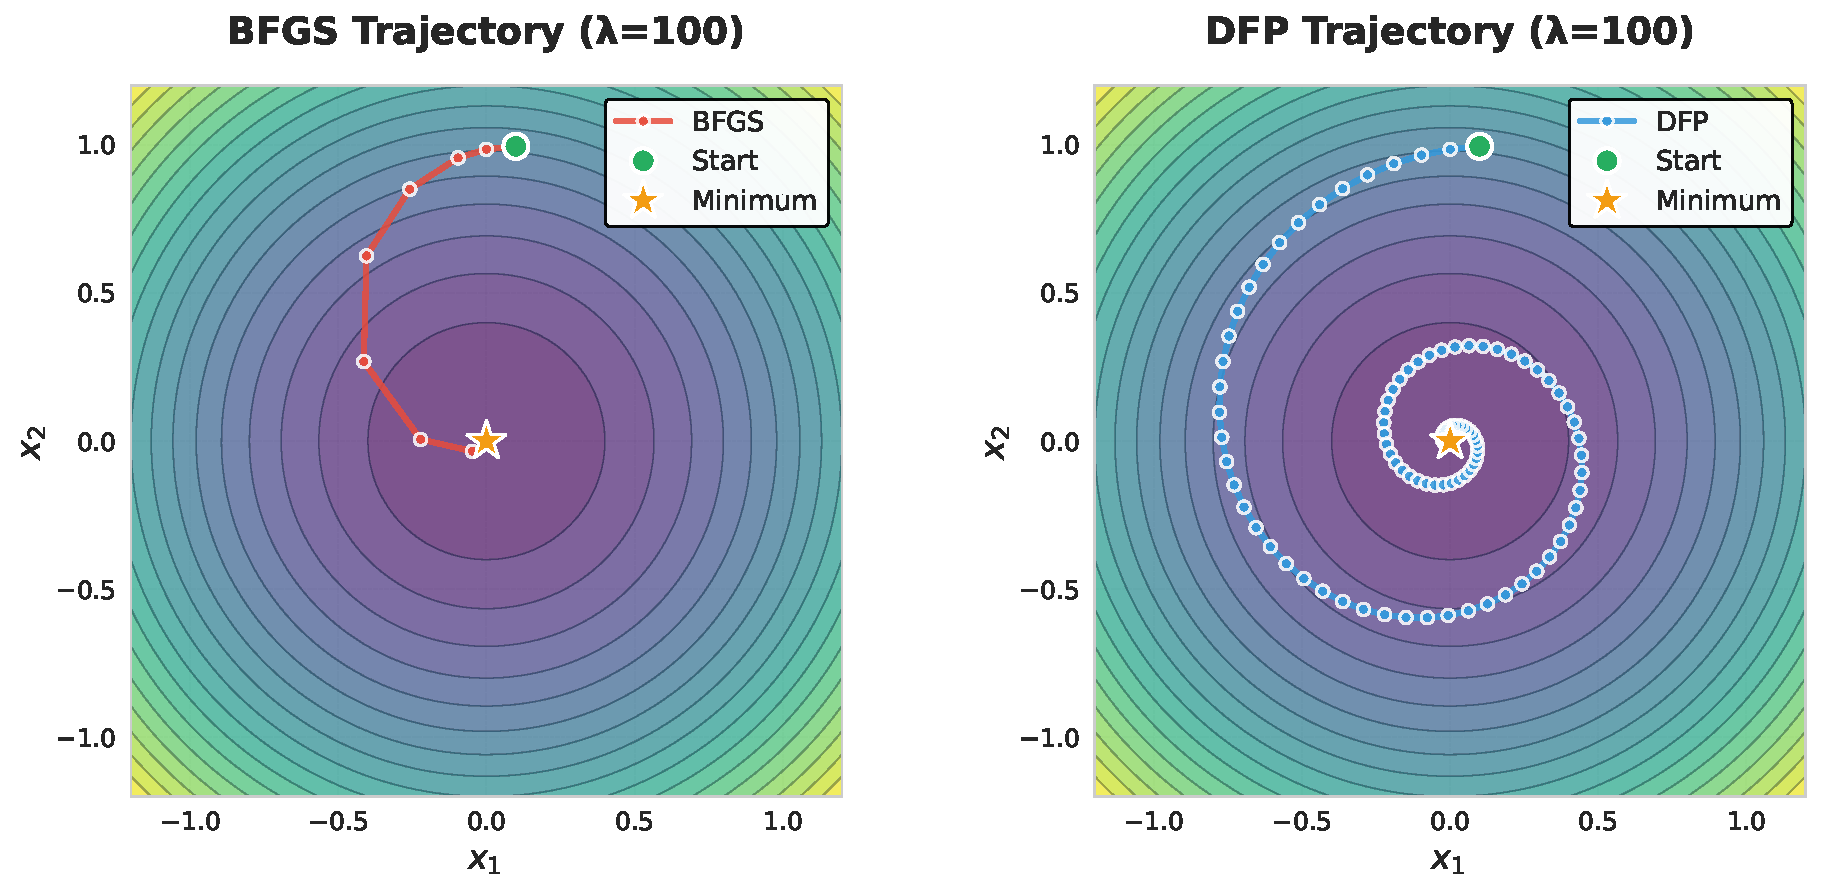
\includegraphics[width=\textwidth]{../imgs/quasi_newton/bfgs_vs_dfp_100.pdf}
    \caption{
        \ifEn
            Iterative trajectories for BFGS and DFP methods when $\lambda_1 = 100$. BFGS converges in 10 iterations while DFP requires 107 iterations, showing BFGS's superior efficiency for large eigenvalue errors.
        \else
            $\lambda_1 = 100$ における BFGS と DFP の反復軌跡。BFGS は 10 回で収束する一方、DFP は 107 回を要し、固有値誤差が大きい場合に BFGS が優位であることを示す。
        \fi
    }
    \label{fig:bfgs_dfp_100}
\end{figure}

\begin{figure}[t]
    \centering
    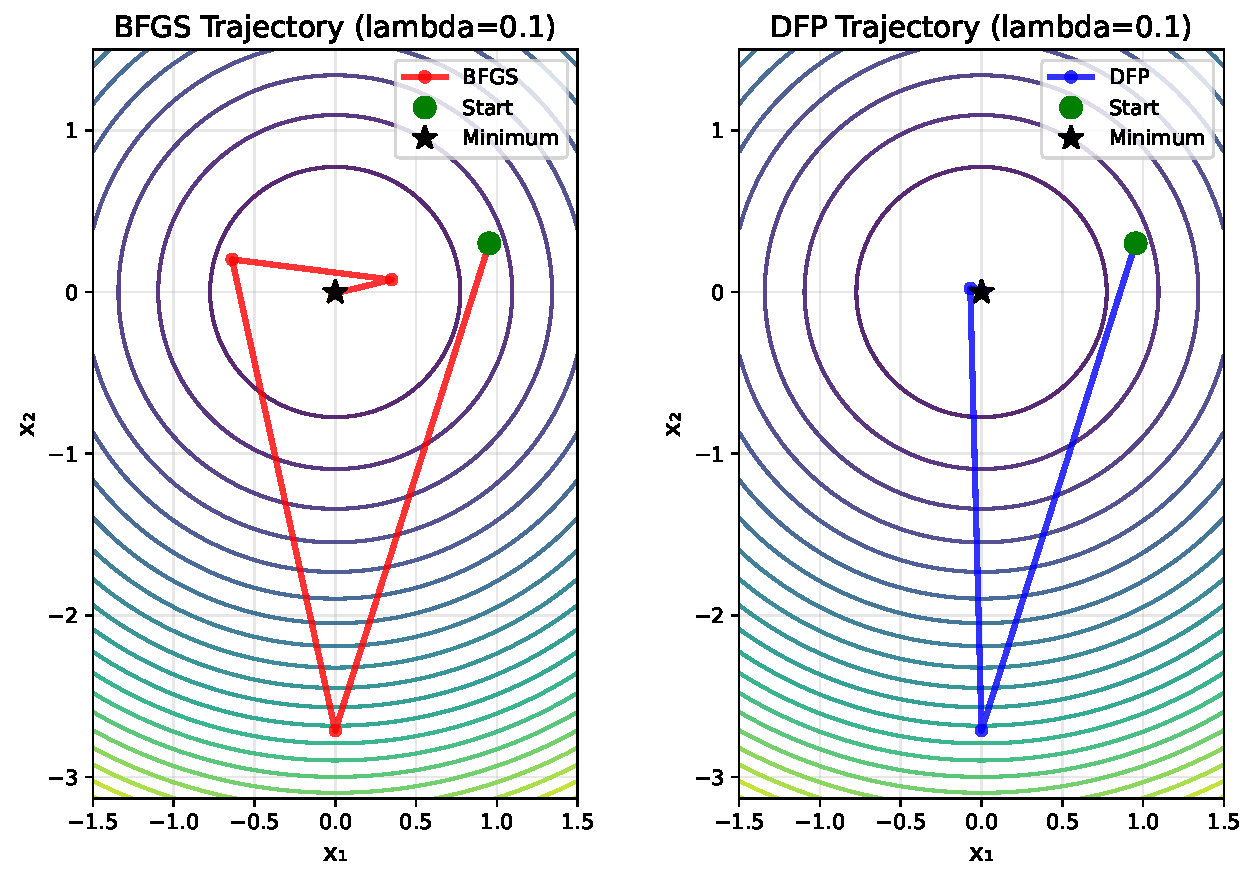
\includegraphics[width=\textwidth]{../imgs/quasi_newton/bfgs_vs_dfp_0.1.pdf}
    \caption{
        \ifEn
            Iterative trajectories for BFGS and DFP methods when $\lambda_1 = 0.1$. Both methods converge quickly, with DFP slightly faster than BFGS, demonstrating the symmetric behavior when eigenvalues are underestimated.
        \else
            $\lambda_1 = 0.1$ における BFGS と DFP の反復軌跡。どちらも素早く収束し、DFP が BFGS よりわずかに速い。固有値が過小評価された場合の対称的な振る舞いを示している。
        \fi
    }
    \label{fig:bfgs_dfp_0p1}
\end{figure}

\ifEn
    \subsubsection{Analysis and Discussion}
\else
    \subsubsection{解析と議論}
\fi

\ifEn
    The numerical results reveal a striking asymmetry between BFGS and DFP.
    When $\lambda_1 > 1$ (i.e., the initial Hessian approximation overestimates the true Hessian curvature), BFGS demonstrates significantly better efficiency.
    Conversely, when $\lambda_1 < 1$ (i.e., the initial Hessian approximation underestimates the true curvature), DFP performs slightly better than BFGS, though the difference is modest.
    This trend reversal is predicted by the theoretical symmetry between the two methods, but the magnitude of the difference is notable.
\else
    数値結果は BFGS と DFP の間に顕著な非対称性があることを示す。
    $\lambda_1 > 1$ のとき、すなわち初期ヘッセ近似が真の曲率を過大評価する場合、BFGS は大幅に高い効率を示す。
    逆に $\lambda_1 < 1$ のとき、すなわち初期ヘッセ近似が真の曲率を過小評価する場合、DFP は BFGS よりわずかに良いが、その差は小さい。
    この傾向の逆転は理論的な対称性から予測されるが、差の大きさは注目に値する。
\fi

\ifEn
    \paragraph{Asymmetry in Hessian Correction}
\else
    \paragraph{ヘッセ補正の非対称性}
\fi

\ifEn
    The asymmetry of the performance arises from a fundamental difference in how these two methods correct erroneous eigenvalues.
    The core insight is that correcting erroneously large eigenvalues is more critical than correcting erroneously small ones.

    When a Hessian eigenvalue is overestimated, the algorithm takes steps that are too conservative, resulting in slow progress toward the minimum. Correcting such errors requires the update formula to reduce these large eigenvalues toward one.
    The BFGS update is highly effective at this task.

    In contrast, when a Hessian eigenvalue is underestimated, the algorithm takes steps that are slightly too aggressive, but the error is self-correcting.
    Subsequent gradient computations provide information that helps refine the approximation.
    Thus, correcting underestimated eigenvalues is inherently easier and requires fewer iterations.

    The DFP update struggles with large eigenvalues.
    In the worst case, it can reduce a large eigenvalue by only a small amount per iteration, potentially requiring as many iterations as the magnitude of the eigenvalue itself.
    This explains why DFP's performance degrades catastrophically as $\lambda_1$ increases beyond one.
\else
    性能の非対称性は、両手法が誤った固有値を補正する仕方の根本的な違いに起因する。
    核心的な洞察は、過大な固有値の補正が過小な固有値の補正より重要であるという点である。

    ヘッセ固有値が過大評価されると、アルゴリズムは過度に保守的なステップを取り、最小点への進みが遅くなる。この誤差を補正するには、更新公式が大きな固有値を 1 へ縮小する必要がある。
    BFGS 更新はこの作業に非常に効果的である。

    一方、ヘッセ固有値が過小評価される場合、アルゴリズムはやや攻撃的なステップを取るが、誤差は自己修正的である。
    その後の勾配計算が近似の改善に役立つ情報を提供する。
    そのため過小評価の補正は本質的に容易で、必要な反復回数も少ない。

    DFP 更新は大きな固有値の補正が苦手である。
    最悪の場合、1反復で大きな固有値をわずかしか減らせず、固有値の大きさに匹敵する回数の反復が必要になることがある。
    このことが $\lambda_1$ が 1 を超えて増加するにつれて DFP の性能が急激に悪化する理由である。
\fi

\ifEn
    \paragraph{Practical Implications}
\else
    \paragraph{実用上の含意}
\fi

\ifEn
    These findings provide strong empirical justification for the widespread practical preference for BFGS over DFP.
    The analysis of Powell's simple quadratic problem yields deep insights about quasi-Newton methods' behavior far from the solution, where most computational effort is expended.
    The superior efficiency of BFGS in correcting erroneous Hessian approximations makes it the algorithm of choice for robust and efficient unconstrained optimization.
\else
    これらの知見は、実務で BFGS が DFP より広く選好されることに強い経験的根拠を与える。
    Powell の単純な二次問題の解析は、計算量の大半が費やされる解から遠い領域での準ニュートン法の挙動に深い洞察を与える。
    誤ったヘッセ近似の補正における BFGS の優位性は、ロバストで効率的な無制約最適化のための第一選択としての地位を支えている。
\fi

\ifEn
    \subsection{Limited Memory BFGS (L-BFGS)}
\else
    \subsection{限定記憶 BFGS (L-BFGS)}
\fi

\ifEn
    Limited-memory quasi-Newton methods extend classical quasi-Newton methods to large-scale optimization problems.
    In standard quasi-Newton methods, the approximate Hessian or inverse Hessian matrix is stored and updated as a dense matrix, requiring $\mathcal{O}(n^2)$ memory for $n$ variables.
\else
    限定記憶準ニュートン法は、古典的な準ニュートン法を大規模最適化問題へ拡張する手法である。
    標準的な準ニュートン法では近似ヘッセ行列またはその逆行列を密行列として保存し更新するため、$n$ 変数に対して $\mathcal{O}(n^2)$ のメモリを要する。
\fi

\ifEn
    The L-BFGS method~\citep{liuLimitedMemoryBFGS1989a}, which is based on the BFGS update, avoids storing the full matrix explicitly.
    Instead, it maintains only the most recent $m$ vector pairs $\{(s_i,y_i)\}$.
    This reduces the storage requirement to $\mathcal{O}(nm)$, which is a dramatic improvement when $m$ is a small constant (typically $m\le 10$).
\else
    BFGS 更新に基づく L-BFGS 法~\citep{liuLimitedMemoryBFGS1989a} は、行列全体を明示的に保存しない。
    代わりに最新の $m$ 組のベクトル対 $\{(s_i,y_i)\}$ のみを保持する。
    これにより記憶量は $\mathcal{O}(nm)$ に減少し、$m$ が小さな定数(通常 $m\le 10$) のとき大幅な改善となる。
\fi

\ifEn
    Throughout this subsection, we work with a finite sequence of matrices
\else
    本小節では次の有限列の行列を扱う。
\fi
\begin{equation*}
    H_0, H_1, \dots, H_m,
\end{equation*}
\ifEn
    where $H_\ell$ denotes the inverse Hessian approximation obtained after $\ell$ BFGS updates applied to a given initial matrix $H_0$.
    Note that this is not the same as the iterates in an optimization algorithm. Here, we focus solely on the structure of the BFGS updates.
\else
    ここで $H_\ell$ は初期行列 $H_0$ に対して $\ell$ 回の BFGS 更新を適用して得られる逆ヘッセ近似を表す。
    これは最適化アルゴリズムの反復点とは異なる点に注意する。本小節では BFGS 更新の構造のみに注目する。
\fi

\ifEn
    \subsubsection{Compact Representation of the Inverse BFGS Update}
\else
    \subsubsection{逆 BFGS 更新のコンパクト表現}
\fi

\ifEn
    Let $\{(s_i,y_i)\}_{i=0}^{m-1}$ be the stored correction pairs, and define
\else
    保存された補正対 $\{(s_i,y_i)\}_{i=0}^{m-1}$ を用い、次を定義する。
\fi
\begin{equation*}
    \rho_i = \frac{1}{y_i^\top s_i}, \qquad
    V_i = I - \rho_i y_i s_i^\top.
\end{equation*}
\ifEn
    The inverse BFGS update can be expressed as
\else
    逆 BFGS 更新は次のように表される。
\fi
\begin{equation*}
    H_{i+1} = V_i^\top H_i V_i + \rho_i s_i s_i^\top,
\end{equation*}
\ifEn
    for $i = 0,\dots,m-1$.
    By recursively expanding this relation, we obtain the compact representation
\else
    ここで $i = 0,\dots,m-1$ である。
    この関係を再帰的に展開すると次のコンパクト表現が得られる。
\fi
\begin{equation*}
    H_m
    =
    V_{m-1}^\top \cdots V_0^\top H_0 V_0 \cdots V_{m-1}
    +
    \sum_{j=0}^{m-1}
    (V_{m-1}^\top \cdots V_{j+1}^\top)
    \rho_j s_j s_j^\top
    (V_{j+1} \cdots V_{m-1}),
\end{equation*}
\ifEn
    where $H_0$ denotes the chosen initial inverse Hessian approximation, typically a scaled identity matrix.
\else
    ここで $H_0$ は選ばれた初期逆ヘッセ近似であり、通常はスケールされた単位行列である。
\fi

\ifEn
    \subsubsection{Two-Loop Recursion}
\else
    \subsubsection{二重ループ再帰}
\fi

\ifEn
    The compact representation above can be applied to any vector $q$ without explicitly forming $H_m$.
    Let $r = H_m q$.
    Exploiting the associative structure of the matrix products, this operation can be carried out using two short loops of length $m$, leading to the well-known L-BFGS two-loop recursion~\citep[Algorithm 7.4]{nocedal1999numerical}.
    This algorithm requires $\mathcal{O}(md)$ arithmetic operations and $\mathcal{O}(md)$ storage, where $d$ denotes the problem dimension.
\else
    上のコンパクト表現は、$H_m$ を明示的に形成せずに任意のベクトル $q$ に適用できる。
    $r = H_m q$ とおく。
    行列積の結合性を利用すると、この計算は長さ $m$ の短いループを二回回すだけで実行でき、よく知られた L-BFGS の二重ループ再帰につながる~\citep[Algorithm 7.4]{nocedal1999numerical}。
    このアルゴリズムは $\mathcal{O}(md)$ の演算量と $\mathcal{O}(md)$ の記憶量を要する。ここで $d$ は問題次元である。
\fi

\subfile{999_two_loop_recursion.tex}

\ifEn
    Now, we verify that the output of the two-loop recursion algorithm indeed computes $r = H_m q$.
\else
    次に、この二重ループ再帰の出力が確かに $r = H_m q$ を計算していることを確認する。
\fi
\begin{proposition}
    \ifEn
        The output of the two-loop recursion algorithm satisfies $r = H_m q$.
    \else
        二重ループ再帰アルゴリズムの出力は $r = H_m q$ を満たす。
    \fi
\end{proposition}
\begin{proof}
    \ifEn
        In the backward recursion, for $i = m-1, m-2, \dots, 0$, from the input vector $q^{(m)} \coloneqq q$, the algorithm computes
    \else
        逆方向の再帰では、$i = m-1, m-2, \dots, 0$ に対して入力ベクトル $q^{(m)} \coloneqq q$ から次を計算する。
    \fi
    \begin{equation*}
        \alpha_i   = \rho_i s_i^\top q^{(i+1)}, \qquad
        q^{(i)} \coloneqq q^{(i+1)} - \alpha_i y_i.
    \end{equation*}
    \ifEn
        Substituting the definition of $\alpha_i$ and using the definition of $V_i$, we find
    \else
        $\alpha_i$ の定義を代入し $V_i$ の定義を用いると
    \fi
    \begin{equation*}
        q^{(i)} = q^{(i+1)} - \rho_i \left(s_i^\top q^{(i+1)}\right) y_i = \left(I - \rho_i y_i s_i^\top\right) q^{(i+1)} = V_i q^{(i+1)}.
    \end{equation*}
    \ifEn
        Thus, for all $i = 0, 1, \dots, m-1$, we have
    \else
        よってすべての $i = 0, 1, \dots, m-1$ に対して
    \fi
    \begin{equation*}
        q^{(i)} = V_i V_{i+1} \cdots V_{m-1} q.
    \end{equation*}
    \ifEn
        Then, the algorithm applies the initial inverse Hessian approximation:
    \else
        次にアルゴリズムは初期逆ヘッセ近似を適用する。
    \fi
    \begin{equation*}
        r^{(0)} = H_0 q^{(0)} = H_0 V_0 V_1 \cdots V_{m-1} q.
    \end{equation*}
    \ifEn
        Next, for $i = 0, 1, \dots, m-1$, the forward recursion computes
    \else
        次に $i = 0, 1, \dots, m-1$ に対して前方向の再帰は次を計算する。
    \fi
    \begin{equation*}
        \beta_i     = \rho_i y_i^\top r^{(i)}, \qquad
        r^{(i+1)}   = r^{(i)} + s_i \left(\alpha_i - \beta_i\right).
    \end{equation*}
    \ifEn
        Substituting the definitions of $\alpha_i$, $\beta_i$, and $q^{(i+1)}$, we have
    \else
        $\alpha_i$, $\beta_i$, $q^{(i+1)}$ の定義を代入すると
    \fi
    \begin{align*}
        r^{(i+1)}
         & =
        r^{(i)} + \rho_i s_i s_i^\top \left(V_{i+1} V_{i+2} \cdots V_{m-1}\right) q - \rho_i s_i y_i^\top r^{(i)}            \\
         & = \left(I- \rho_i y_i s_i^\top\right) r^{(i)} + \rho_i s_i s_i^\top \left(V_{i+1} V_{i+2} \cdots V_{m-1}\right) q \\
         & =
        V_i^\top r^{(i)}
        +
        \rho_i s_i s_i^\top
        \left(V_{i+1} V_{i+2} \cdots V_{m-1}\right) q.
    \end{align*}
    \ifEn
        By recursively expanding this relation from the initial value $r^{(0)} = H_0 q^{(0)}$, we obtain
    \else
        初期値 $r^{(0)} = H_0 q^{(0)}$ からこの関係を再帰的に展開すると
    \fi
    \begin{equation*}
        r^{(m)}
        =
        V_{m-1}^\top \cdots V_0^\top H_0 V_0 \cdots V_{m-1} q
        +
        \sum_{j=0}^{m-1}
        (V_{m-1}^\top \cdots V_{j+1}^\top)
        \rho_j s_j s_j^\top
        (V_{j+1} \cdots V_{m-1}) q,
    \end{equation*}
    \ifEn
        which matches the compact representation of $H_m$ applied to $q$, completing the proof.
    \else
        となり、$H_m$ のコンパクト表現を $q$ に適用した式と一致する。これで証明が完了する。
    \fi
    \myQED
\end{proof}

\ifEn
    Thus, the two-loop recursion exactly evaluates the action of $H_m$ on a vector while avoiding explicit matrix construction, achieving both mathematical rigor and computational efficiency.
\else
    従って二重ループ再帰は、行列を明示的に構成せずに $H_m$ の作用を正確に評価し、数学的厳密さと計算効率の両方を実現する。
\fi

\ifEn
    \subsubsection{Initial Step Size}
\else
    \subsubsection{初期スケーリング}
\fi

\ifEn
    A crucial component of the L-BFGS method is the choice of the initial matrix $H_0$.
    A widely used and well-justified option is a scaled identity,
\else
    L-BFGS 法の重要な要素は初期行列 $H_0$ の選択である。
    広く使われ、十分に正当化された選択はスケールされた単位行列である。
\fi
\begin{equation*}
    H_0 = \gamma I,
\end{equation*}
\ifEn
    where the scaling parameter is chosen as
\else
    ここでスケーリング係数は次で選ぶ。
\fi
\begin{equation*}
    \gamma = \frac{s_{m-1}^\top y_{m-1}}{y_{m-1}^\top y_{m-1}}.
\end{equation*}
\ifEn
    This choice is motivated by the relationship between the approximate inverse Hessian and the local curvature of the objective function~\citep{liuLimitedMemoryBFGS1989a,shannoMatrixConditioningNonlinear1978}.
    To justify this scaling, assume that the objective function $f$ is twice continuously differentiable and consider the mean Hessian along the most recent step:
\else
    この選択は近似逆ヘッセ行列と目的関数の局所曲率の関係に基づく~\citep{liuLimitedMemoryBFGS1989a,shannoMatrixConditioningNonlinear1978}。
    このスケーリングを正当化するため、目的関数 $f$ が二回連続微分可能であると仮定し、最新のステップに沿った平均ヘッセ行列を考える。
\fi
\begin{equation*}
    \bar{G} = \int_0^1 \nabla^2 f(x + \tau s_{m-1}) \mathrm{d}\tau,
\end{equation*}
\ifEn
    where $s_{m-1}$ denotes the most recent displacement.
    By the mean value theorem,
\else
    ここで $s_{m-1}$ は最新の変位を表す。
    平均値の定理より
\fi
\begin{equation*}
    y_{m-1}
    =
    \nabla f(x+s_{m-1}) - \nabla f(x)
    =
    \bar{G} s_{m-1}.
\end{equation*}
\ifEn
    Using this relation, the scaling factor can be written as
\else
    この関係を用いるとスケーリング係数は次のように書ける。
\fi
\begin{equation*}
    \frac{s_{m-1}^\top y_{m-1}}{y_{m-1}^\top y_{m-1}}
    =
    \frac{(\bar{G}^{1/2} s_{m-1})^\top (\bar{G}^{1/2} s_{m-1})}
    {(\bar{G}^{1/2} s_{m-1})^\top \bar{G} (\bar{G}^{1/2} s_{m-1})},
\end{equation*}
\ifEn
    which is a Rayleigh quotient.
    If $\bar{G}^{1/2} s_{m-1}$ happens to be an eigenvector of $\bar{G}$, then the reciprocal of this quantity equals the corresponding eigenvalue.
\else
    これは Rayleigh 商である。
    もし $\bar{G}^{1/2} s_{m-1}$ が $\bar{G}$ の固有ベクトルであれば、この量の逆数は対応する固有値に等しい。
\fi

\ifEn
    Moreover, the choice of $\gamma$ coincides with the short step size of the Barzilai--Borwein method~\citep{barzilaiTwoPointStepSize1988}, highlighting a close connection between L-BFGS initialization and classical step-length selection strategies.
    This observation further supports the effectiveness of the scaled-identity initialization in practice.
\else
    さらに $\gamma$ の選択は Barzilai--Borwein 法の短ステップサイズ~\citep{barzilaiTwoPointStepSize1988} と一致し、L-BFGS の初期化と古典的なステップ長選択戦略の密接な関係を示している。
    この観察は、実用におけるスケール単位行列初期化の有効性をさらに支持する。
\fi

\ifSubfilesClassLoaded{
    \bibliographystyle{plainnat}
    \bibliography{../L-BFGS.bib}
}{}

\end{document}